\documentclass[journal,twoside,web]{ieeecolor}
\usepackage{generic}
\usepackage{cite}
\usepackage{amsmath,amssymb,amsfonts}
\usepackage{algorithmic}
\usepackage{graphicx}
\usepackage{algorithm,algorithmic}
\usepackage{hyperref}
\hypersetup{hidelinks=true}
\usepackage{textcomp}
% added packages
\usepackage{verbatim}
\usepackage{subcaption}
\graphicspath{{Fig/}}
\usepackage{booktabs}
\usepackage[flushleft]{threeparttable}
\usepackage{placeins}
\usepackage{graphicx} % For resizing tables

%\usepackage{natbib}
\usepackage[flushleft]{threeparttable}
\usepackage{placeins}

\def\BibTeX{{\rm B\kern-.05em{\sc i\kern-.025em b}\kern-.08em
    T\kern-.1667em\lower.7ex\hbox{E}\kern-.125emX}}
\markboth{\hskip25pc IEEE TRANSACTIONS AND JOURNALS TEMPLATE}
{Author \MakeLowercase{\textit{et al.}}: Title}
\begin{document}
\title{Supplementary material for\\ DruGNNosis-MoA: Elucidating Drug Mechanisms as Etiological or Palliative with Graph Neural Networks Employing a Large Language Model}
\author{
%Brettler Liad, 
%Berman Eden,
%Jagodnik Kathleen M.,
%and 
%Bartal Alon
\thanks{
%This paragraph of the first footnote will contain the date on 
%All authors are with the The School of Business Administration, Bar-Ilan University, Ramat-Gan, 5290002, Israel (e-mail: alon.bartal@biu.ac.il).
}
}

\maketitle

%Full names of authors are preferred in 

%the author field, but are not required.

%Put a space between authors' initials.

%The abstract must be between 150--250 words. 

% three or four different keywords or phrase

%---------------------------------------------------------------------
\appendices
%---------------------------------------------------------------------
%\begin{appendices}

\setcounter{figure}{0}
\renewcommand\thefigure{S\arabic{figure}} % Redefine table numbering style

%-------------------
\section{Supplementary Figures}
%-------------------
\begin{figure}[h!]
    \centering
    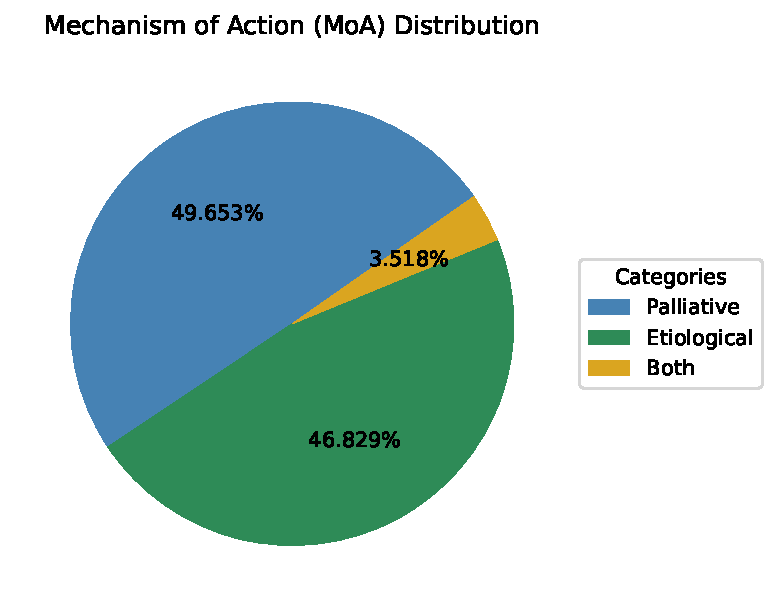
\includegraphics[width=\linewidth]{Figures/EvsP.pdf}
    \caption{Distribution of drug mechanisms of action. The number of etiological and palliative drugs is well balanced, with 47.423\% (957) being etiological, and 48.761\% (984) being palliative.
    Only a small percentage (3.816\%, 77) of drugs exhibit both mechanisms.}
    \label{fig:EvsP}
\end{figure}

%-------------------

\begin{figure}[h!]
    \centering
    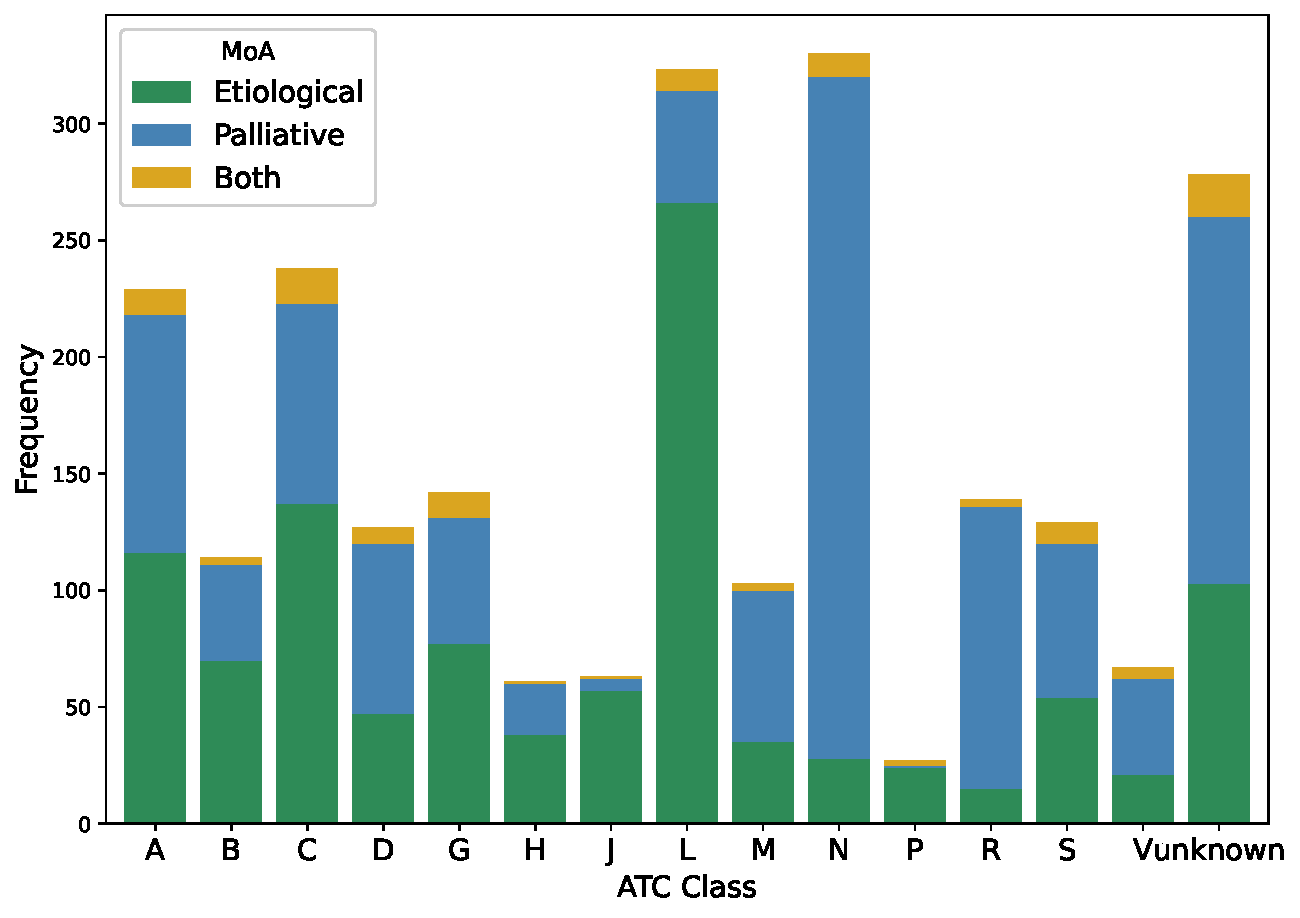
\includegraphics[width=\linewidth]{Figures/EPvsATC.pdf}
    \caption{ Distribution of drug mechanisms across Anatomical Therapeutic Chemical (ATC) classes.
    Each ATC class has a unique distribution of drug mechanisms.
    Some classes, e.g., `J', `L', and `P', are mainly associated with drugs having etiological mechanisms.
    In contrast, classes like 'N' and `R' are primarily associated with drugs having palliative mechanisms.
    The remaining classes generally exhibit a balance between drugs with etiological and palliative mechanisms.
    ATC Class Definitions:
   ``A": Alimentary tract and metabolism;
   ``B": Blood and blood forming organs;
   ``C": Cardiovascular system;
   ``D": Dermatologicals;
   ``G": Genito urinary system and sex hormones;
   ``H": Systemic hormonal preparations, excluding sex hormones and insulins;
   ``J": Antiinfectives for systemic use;
   ``L": Antineoplastic and immunomodulating agents;
   ``M": Musculo-skeletal system;
   ``N": Nervous system;
   ``P": Antiparasitic products, insecticides and repellents;
   ``R": Respiratory system;
   ``S": Sensory organs;
   ``V": Various;
   "Unknown": Drug entries that do not have an ATC class assigned to them in DrugBank.
    }
    \label{fig:EPvsATC}
\end{figure}

%-------------------

\begin{figure}
\centering
\begin{subfigure}{\linewidth}
   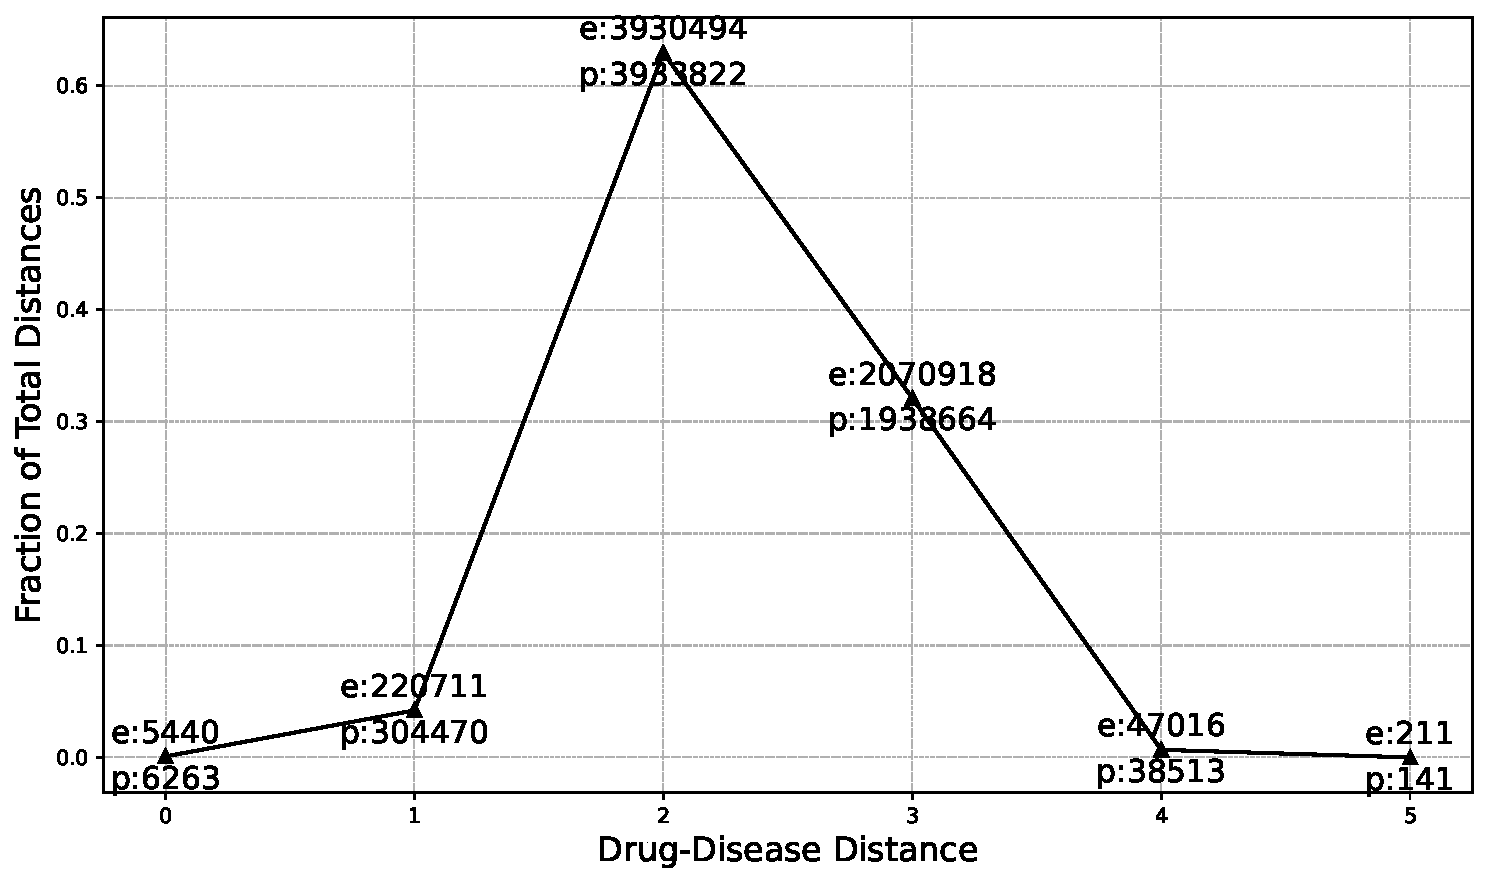
\includegraphics[width=\linewidth]{Figures/Yildrim_all_shortest_distance.pdf}
   \caption{\textbf{All vs. All (Comprehensive) Method:} Calculates and counts the shortest distance between each drug and disease pair, considering each occurrence of the drug in multiple paths.
   A drug–disease distance of 0 indicates that the drug and the disease nodes are directly connected.
   According to the technique proposed in [5], distances of 0 and 1 hold statistical significance and are indicative of etiological drug mechanisms; however, our results do not support this finding.}
   \label{fig:yildirim1}
\end{subfigure}
\begin{subfigure}{\linewidth}
   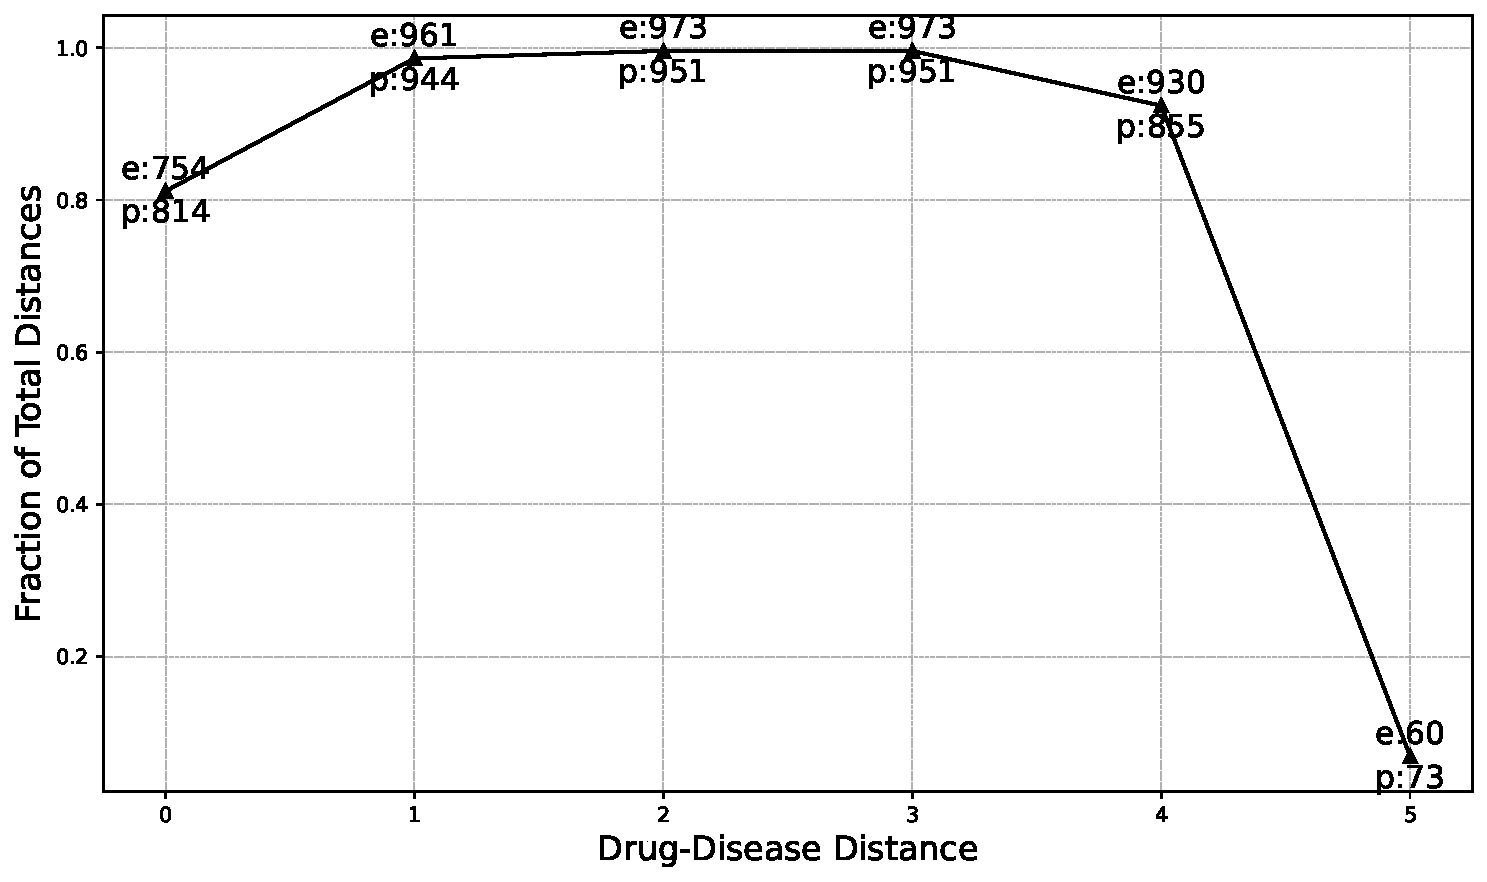
\includegraphics[width=\linewidth]{Figures/Yildrim_ALL_unique_drug_count_shortest_distance.pdf}
   \caption{\textbf{All vs. All (Unique) Method:} 
   Calculates the shortest distances between each drug and disease pair using a distinct counting mechanism. A drug is counted only once at each unique distance, regardless of how many times it appears at that distance. This ensures a balanced representation of drug applications relative to distance, preventing overemphasis on drugs appearing multiple times at the same distance.}
   \label{fig:yildirim2}
\end{subfigure}
\begin{subfigure}{\linewidth}
   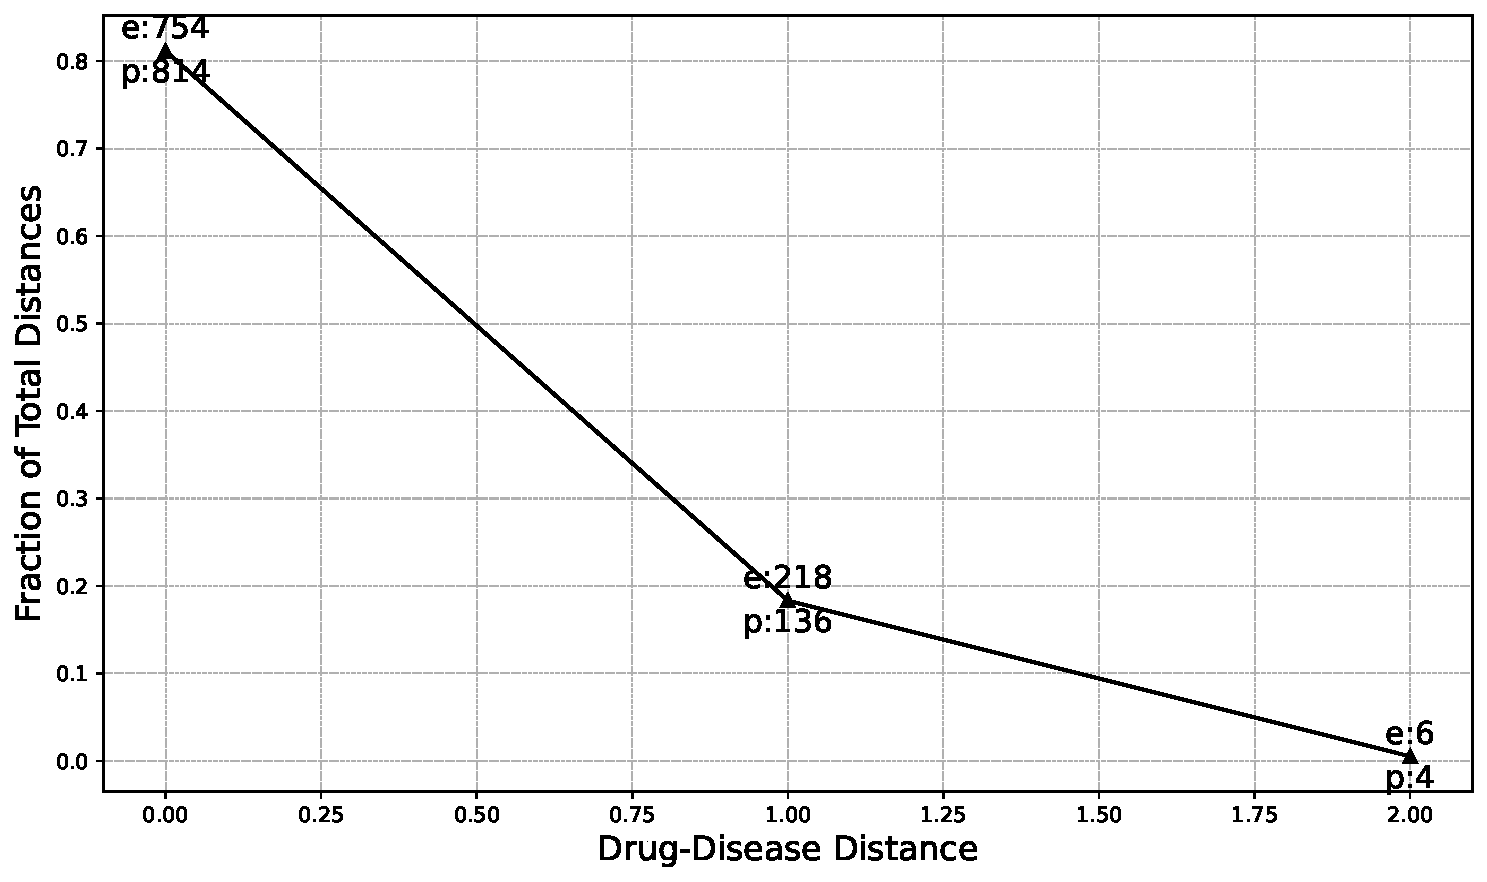
\includegraphics[width=\linewidth]{Figures/Yildrim_unique_minimum_shortest_distance.pdf}
   \caption{\textbf{Unique Minimum Shortest Distance Method:} 
    For each drug, we identified its distance to a disease (presenting distances $\leq 2$). 
    We retained only one unique distance per drug.
   }
   \label{fig:yildirim3}
\end{subfigure}
\caption{Three methods for calculating drug-disease distances.
Abbreviations: e = Etiological, p = Palliative. 
Numerical values represent the number of paths between drug and disease pairs at a specific distance. 
The fraction for each distance (path length) is calculated by dividing the number of occurrences of that specific path length by the total number of paths in the dataset.
This measures how common each distance is, relative to all possible paths.}
\label{fig:yildirim}
\end{figure}

%-------------------

\begin{figure}[h!]
\centering
   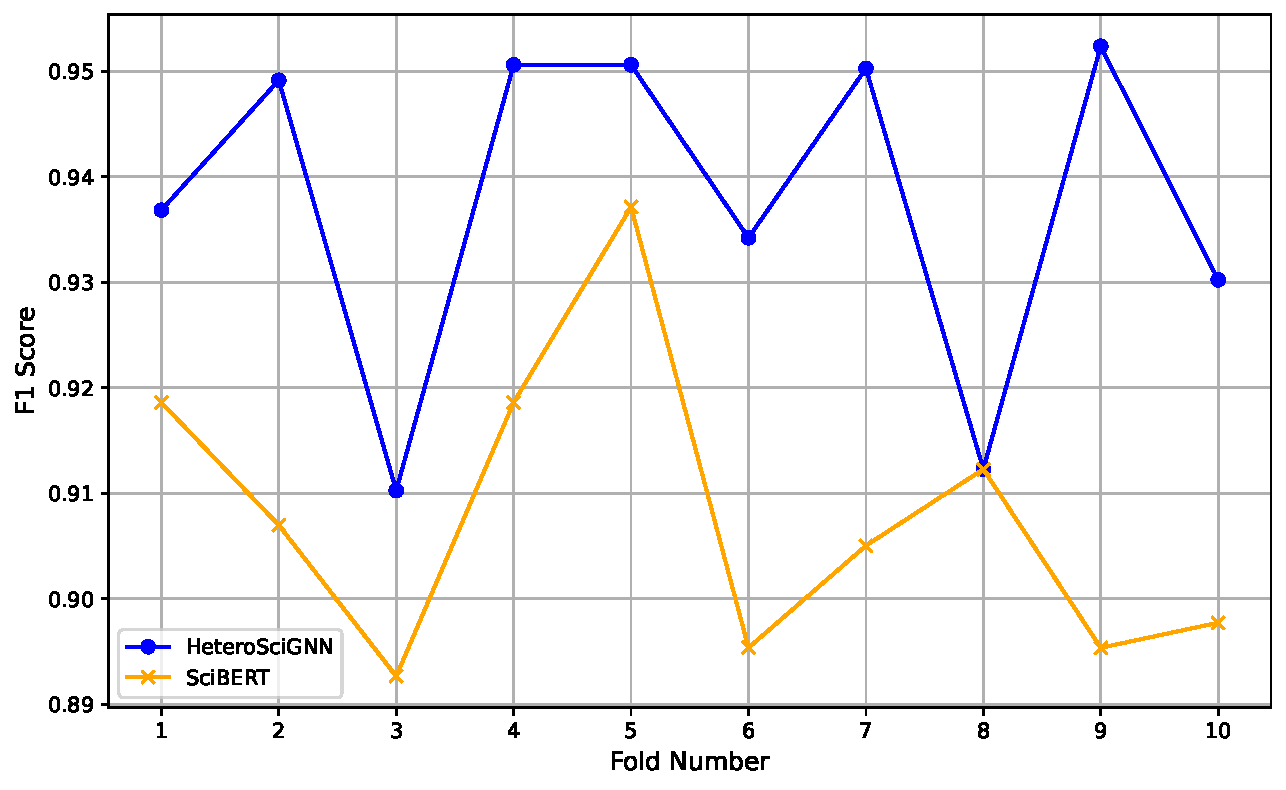
\includegraphics[width=\linewidth]{Figures/Comparison_F1_Scores_2_models.pdf}
   \caption{
    Comparison of F1-scores between the DruGNNosis-MoA and our fine-tuned SciBERT models.
   Each point on the lines corresponds to the F1-score obtained for that particular fold of the cross-validation.
   DruGNNosis-MoA model outperformed our fine-tuned SciBERT on a fold-by-fold basis.}
\label{fig:fscore1}
\end{figure}

%-------------------
\begin{figure}[h!]
    \centering
    \includegraphics[width=\linewidth]{Figures/LDA.png}
    \caption{LDA topic modeling results.
    The left panel shows the Intertopic Distance Map, where each bubble represents a topic identified by the LDA model. 
    The size of the bubble indicates the proportion of tokens attributed to the topic. 
    The spatial separation of Topic 2 from other topics suggests its distinctiveness in terms of term usage. 
    The right panel displays the Top-30 Most Relevant Terms for Topic 2, ranked by a relevance metric ($\lambda = 0.28$) that balances term specificity and frequency. Prominent terms for Topic 2 include `histamine,' `norepinephrine,' and `allergic,' indicating a focus on treatments related (palliative) to allergic responses and histamine pathways, such as antihistamines and adrenergic drugs. 
    The red bars represent the estimated frequency of terms within Topic 2, while the blue bars represent their overall frequency across all topics.}
    \label{fig:LDA}
\end{figure}


\newpage

\clearpage

%-------------------
\section{Supplementary Tables}
\label{sec11}
%-------------------

%-------------------
%{Supplementary Table S1}
%-------------------
\subsection{Supplementary Table S1} 
Table S1 can be accessed through: 
\url{https://github.com/Anonymousv123/DruGNNosis-MoA/tree/main/Supplementary}
%\url{https://github.com/bartala/PalliativEtiological/tree/main/Supplementary}.
Tab 1 contains drug mechanism annotations.
Tab 2 contains example drug mechanism.


%-------------------
%{Supplementary Table S2}
%-------------------
\begin{table}[h!]
\centering
\begin{threeparttable}
\caption*{Table S2: Training configurations of baseline GNNs.}
\label{tbl:cv_scores}
\begin{tabular}{@{\extracolsep\fill} p{0.07\textwidth} p{0.4\textwidth} @{\extracolsep\fill}}
\toprule
Model & Configuration \\
\midrule
SAGEConv & 
    Two SageConv layers, ReLU activation, and an Adam optimizer (learning rate \(5 \times 10^{-4}\)) with gradient clipping at 0.5, and 100 epochs, using EigenVector-based node features.
\\
GATConv+ Fine-tuned SciBERT &  
    Two GATConv layers with multi-head attention followed by ReLU activation. 
    An Adam optimizer with a learning rate of \(5 \times 10^{-4}\) and gradient clipping at 0.5.
    The model was trained over 100 epochs, using fine-tuned SciBERT embeddings as node features.
\\
GATConv & 
    Two GATConv layers with multi-head attention, followed by ReLU activation.
    An Adam optimizer with a learning rate of \(5 \times 10^{-4}\) and gradient clipping at 0.5. The model was trained over 100 epochs using Eigenvector centrality as node features.
\\
GATv2Conv+ Fine-tuned SciBERT &
    Two GATv2Conv layers, utilizing adaptive multi-head attention followed by ReLU activation. 
    An Adam optimizer with a learning rate of \(5 \times 10^{-4}\) and gradient clipping at 0.5.
    The model was trained over 100 epochs, using fine-tuned SciBERT embeddings as node features.
\\
GATv2Conv & 
    Two GATv2Conv layers, utilizing adaptive multi-head attention followed by ReLU activation. 
    An Adam optimizer with a learning rate of \(5 \times 10^{-4}\) and gradient clipping at 0.5. The model was trained over 100 epochs, using Eigenvector centrality as node features.
\\
GraphConv+ Fine-tuned SciBERT & 
    Two GraphConv layers followed by ReLU activation. 
    An Adam optimizer with a learning rate of \(5 \times 10^{-4}\) and gradient clipping at 0.5.
    The model was trained over 100 epochs, using fine-tuned SciBERT embeddings as node features.
\\
GraphConv &  
    Two GraphConv layers to aggregate neighborhood information, followed by ReLU activation. 
    An Adam optimizer with a learning rate of \(5 \times 10^{-4}\) and gradient clipping at 0.5.
    The model was trained over 100 epochs, using Eigenvector centrality as node features.
\\
\bottomrule
\end{tabular}
\begin{tablenotes}
\item Note: Each cross-validation fold used a 90-10 split of the data for training and validation, respectively.
\end{tablenotes}
\end{threeparttable}
\end{table}


%-------------------
\newpage
%-------------------
\begin{figure*}[h!]
    \centering
    \caption*{
    Table S3: Results of LDA topic modeling applied to drug descriptions, intersected with DruGNNosis-MoA predictions. 
    The column headings represent mechanisms of action (MoA), categorized as either palliative or etiological based on the dominant keywords within each topic. 
    Within each topic, keywords are ranked from top to bottom according to their importance in defining that topic.
    The bar charts below the table illustrate the proportion of etiological and palliative labels assigned to each topic by DruGNNosis-MoA. 
    Notably, while each topic contains a mix of labels, the dominant classification generally aligns with the overall keyword categorization.
    LDA identifies underlying topics based on word co-occurrence patterns but does not explicitly classify drugs as etiological or palliative. 
    Instead, the topic compositions provide contextual insights into how drugs are described, which helps interpret DruGNNosis-MoA classifications. 
    While some label overlap exists, the dominant label in each topic typically aligns with DruGNNosis-MoA predictions, suggesting that word usage patterns contribute to model decision-making.
    By aligning DruGNNosis-MoA classifications with LDA topics, we gain insights into how word usage patterns correspond to MoA types, providing a complementary interpretability layer for understanding the model’s classification process. 
    While LDA alone is not an effective classifier, its topic structures reinforce the textual patterns captured by DruGNNosis-MoA.
    Finally, DruGNNosis-MoA was independently evaluated on an unseen test set with high accuracy, confirming that its classifications are robust beyond textual correlations identified by LDA.
    }
    \includegraphics[width=\linewidth]{Figures/table_LDA.pdf}
    \label{fig:moa_distributions}
\end{figure*}



\begin{table}[ht]
\centering
\caption*{Table S4: Performance evaluation for Network-based heuristic methods [5, 9] in accordance with Fig. S3c.}
\label{tab:distance_distribution}
\begin{tabular}{ccc}
\toprule
{Drug–Disease Distance} & {Etiological (e)} & {Palliative (p)} \\
\midrule
0 & 754 & 814 \\
1 & 218 & 136 \\
$\geq 2$ & 6   & 4   \\
\bottomrule
\end{tabular}
\begin{tablenotes}
\item 
To compare the performance of DruGNNosis-MoA to the  network-based heuristic [5, 9], we evaluated the performance of the network-based heuristic [5, 9] based on Fig. S3c.
We predict etiological (e) if drug distance to a disease is 0 or 1.
We predict palliative (p) if drug distance to a disease is 2 or greater.
Next, we define
True Positives (TP): etiological drugs predicted as etiological;
False Positives (FP): palliative drugs predicted as etiological;
False Negatives (FN) etiological drugs predicted as palliative; and
True Negatives (TN): palliative drugs predicted as palliative.
Then, we computed the following measures:
TP = 972,
FP = 950,
FN = 6,
TN = 4,
Precision = 0.506,
Recall = 0.994, and
F1-score = 0.670.

In place of Guney et al.’s [9] proximity measure, which averages the shortest distances between drug targets and disease genes, we use each drug’s minimum drug–disease distance (Fig. S3c) as a proxy. 
This is valid because our graph explicitly models drug–gene and gene–disease connections, so the shortest path from a drug to a disease captures the closest mechanistic link, aligning with the intent of the original proximity score while simplifying computation.
\end{tablenotes}
\end{table}


\newpage


%\end{appendices}

\end{document}
